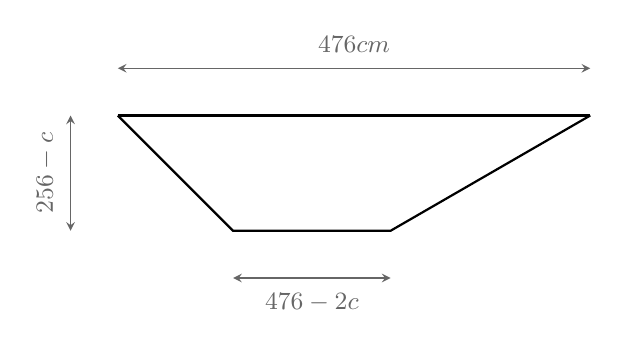
\begin{tikzpicture}[
    scale=2,
    cota/.style={<->, >=stealth, thin, gray!80!black},
    chamada/.style={gray!60, thin, dashed}
]
    % Coordenadas
    \coordinate (D) at (0, 2);
    \coordinate (C) at (3, 2);
    \coordinate (P1) at (0.732, 1.268);
    \coordinate (P2) at (1.732, 1.268);

    % Desenho do Trapézio 2
    \draw[thick] (D) -- (C);                         % Borda livre superior
    \draw[thick] (D) -- (P1) -- (P2) -- (C);         % Linhas de charneira

    % --- EIXO DE COTA HORIZONTAL SUPERIOR (Base Maior) ---
    \def\offsetHTopo{0.3}
    %\draw[chamada] (D) -- (0, 2 + \offsetHTopo + 0.05);
    %\draw[chamada] (C) -- (3, 2 + \offsetHTopo + 0.05);
    \draw[cota] (0, 2 + \offsetHTopo) -- (3, 2 + \offsetHTopo)
        node[midway, above=2pt, font=\small] {$476\text{ cm}$};

    % --- EIXOS DE COTA HORIZONTAIS INFERIORES (Base Menor e Projeções) ---
    \def\offsetHBaixo{0.3}
    \def\yCotaBaixo{1.268 - \offsetHBaixo}

    %\draw[chamada] (0, 1.268) -- (0, \yCotaBaixo - 0.05);
    %\draw[chamada] (P1) -- (0.732, \yCotaBaixo - 0.05);
    %\draw[chamada] (P2) -- (1.732, \yCotaBaixo - 0.05);
    %\draw[chamada] (3, 1.268) -- (3, \yCotaBaixo - 0.05);

    % Trecho esquerdo
    %\draw[cota] (0, \yCotaBaixo) -- (0.732, \yCotaBaixo)
     %   node[midway, below=2pt, font=\small] {$c$};

    % Base menor
    \draw[cota] (0.732, \yCotaBaixo) -- (1.732, \yCotaBaixo)
        node[midway, below=2pt, font=\small] {$476 - 2c$};

    % Trecho direito
    %\draw[cota] (1.732, \yCotaBaixo) -- (3, \yCotaBaixo)
     %   node[midway, below=2pt, font=\small] {$c$};

    % --- EIXO DE COTA VERTICAL (Altura do Trapézio) ---
    \def\offsetV{0.3}
    %\draw[chamada] (D) -- (-\offsetV - 0.05, 2);
    %\draw[chamada] (0, 1.268) -- (-\offsetV - 0.05, 1.268);
    \draw[cota] (-\offsetV, 1.268) -- (-\offsetV, 2)
        node[midway, left=2pt, font=\small, rotate=90, anchor=south] {$256-c$};

\end{tikzpicture}